\section{Chapter Overview}
This chapter consists of the design decisions made to come up with a suitable architecture for implementation, based on the gathered requirements. High-level design, low-level design, design diagrams, UI wireframes have been used to convey how the design goals are expected to be achieved while discussing the reasoning for chosen design decisions.

\section{Design Goals}
% check non-functional requirements as well
% \setlength{\abovecaptionskip}{2pt plus 3pt minus 1pt} % Chosen fairly arbitrarily

\vspace{-4mm}       % remove line spacing after

% \begin{longtable}{|l|p{0.80\linewidth}|}
% \caption{Design Goals of the proposed system} \\
% \hline
% \textbf{Design Goal} & \textbf{Description} \\
% \hline
% \hline
% \end{longtable}

\begin{table}[h!]
\caption{Design Goals of the proposed system}
{\setstretch{1.5} 
\begin{tabular}{|l|p{0.81\linewidth}|}
\hline
\textbf{Design Goal} & \textbf{Description}\\
\hline
Performance & The recommendations matrix \& opinion-mining data can be pre-processed and stored in memory to be used for recommendations. Since ensembled models are expected to be utilized, concurrency would be ideal to get the output from multiple models at the same time. This could cut down the processing time by 4-5 times (based on the number of models that are required to provide recommendations for the given input). \\ 
\hline
Correctness & The correctness \& quality of the output should be of the highest possible level, utilizing all the available data. Explaining why a user is getting the proposed recommendation will ensure that the user isn't misled into wrong purchase decisions. \\ 
\hline
Usability & Since the purpose of the system is to automate and make it easy for the user to explore \gls{nft}s, the usability of the system must be easy for users of all levels of expertise. \\ 
\hline
Scalability & The system may have to support many concurrent user requests in a production environment. The backend should be able to handle this. New data should be able to be added to the system with minimum effort. \\
\hline
Adaptability & Since the utilized Recommendation models may have to be altered based on the available data and user requirements in the future, these models should be able to be easily swapped out for new models while ensuring that the system won't break in the process of upgrading, with minimum changes. \\
\hline
\end{tabular}
}
\end{table}

\section{High-Level Design}
% High-Level Design / System Architecture Design


\subsection{Tiered Architecture}

The system's architecture is depicted in the diagram below. The data, logic and presentation layers are organized in a three-tier architecture.

The research contribution in this system lies in data preprocessing of the \textit{data tier}, recommendations models, and the recommendations diversifier of the \textit{logic tier}.

% drawio file: https://drive.google.com/file/d/1w8qtT_7XMVVc8TiNLongVLBngfqhQPMg/view?usp=sharing

\begin{figure}[h!]
\centering
\frame{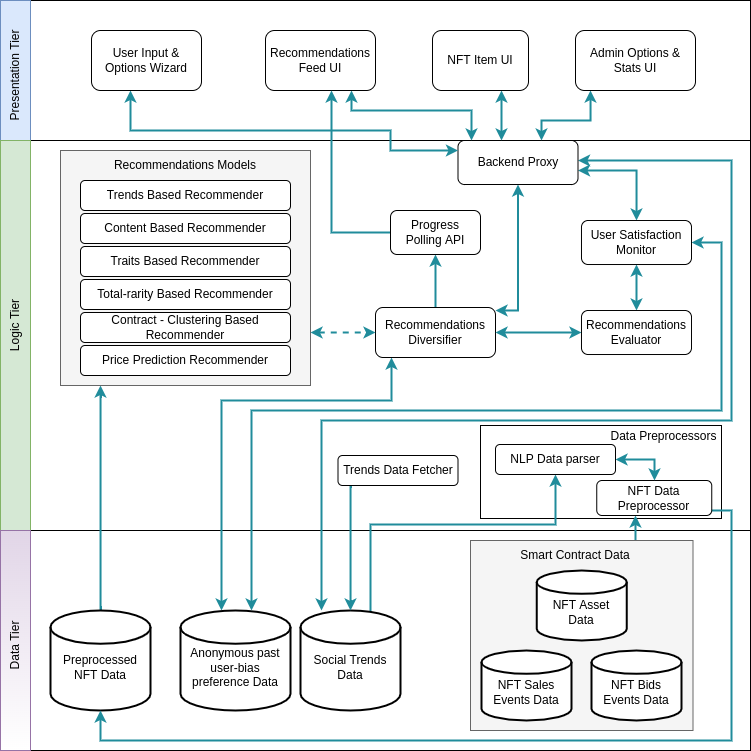
\includegraphics[width=\textwidth]{images/Design/tired-architecture-diagram.png}}
\caption{Three Tiered Architecture \textit{(self-composed)}}
\label{fig:three-tiered-architecuture}
\end{figure}

While the entire architecture is represented in a modular approach for ease of understanding, several backend services are expected to work together in the fashion of a distributed microservices architecture when it comes to implementing the proposed architecture.

The reason for following a microservices architecture is to allow the system to scale while ensuring that points of failure can be easily recognized and taken care of separately. The distributed nature of the system is expected to be seen in the connection between the numerous Recommendations Models and the Recommendations Diversifier. These combined through output pipelines will act as an Ensebled Recommendations System. Although the system will be capable of distributing the load at this point, the expectation with the prototype is to run this in a single machine.

\noindent The purpose of each module that is represented in the above architecture is described below.

% \begin{enumerate}
% \item Data Tier
\subsubsection{Data Tier}
\begin{enumerate}
    \item Smart Contract Data - Data that is retrieved from Blockchain Smart Contracts. For convenience purposes, the data is fetched from the OpenSea API. Contains all the available data of each \gls{nft}.
    \begin{enumerate}
        \item \gls{nft} Asset Data - All the content of each \gls{nft}.
        \item \gls{nft} Sales Events Data - Past sales data from \gls{nft} trading.
        \item \gls{nft} Bids Events Data - All the current bids of each \gls{nft}.  % might not be used for the prototype.
    \end{enumerate}
    \item Social Trends Data - Data gathered from social trends sites (Twitter, news sites, etc.)
    \item Anonymous past user-bias preference Data - Each user's preferred bias is stored anonymously. This can be identified by a user's selection based on their requirement or based on the feedback received for each recommendation. This can be a temporary data store that can be cleared once the user session has ended.
\end{enumerate}

% \item Logic Tier
\subsubsection{Logic Tier}
\begin{enumerate}
    \item Data Preprocessors - The preprocessing code required to modify/ extract required data that is usable for recommendations from all the available data.
    \begin{enumerate}
        \item \gls{nlp} Data parser - Responsible for extracting all the required data from what was collected through data mining techniques.
        \item \gls{nft} Data Preprocessor - Used to modify and separate data that can be utilized from smart contracts and processed trends data.
    \end{enumerate}
    \item Recommendations Models - The various models that are used to provide recommendations based on identified diverse data points.
    % \begin{enumerate}
    %     \item Trends Based Recommender - 
    %     \item Content Based Recommender - 
    %     \item Traits Based Recommender - 
    %     \item Total-rarity Based Recommender - 
    %     \item Contract - Clustering Based Recommender - 
    %     \item Price Prediction Recommender - 
    % \end{enumerate}
    \item Recommendations Diversifier - The module that combines the recommendations produced by all the Recommendations Models, considering the bias.
    \item User Satisfaction Monitor - The feedback received by users will be filtered and updated through this module, to update the moving bias while preserving user anonymity,
    \item Recommendations Evaluator - The module that evaluates the user's satisfaction with the recommendations produced, to separately identify under-performing \& high-performing models.
    \item Progress Polling API - The web-polling API that will be used to update the progress of recommendations generation in the frontend.
    \item Backend Proxy - The interface that exposes the backend services to the frontend.
    \item Trends Data Fetcher - Fetch global trends data from social \gls{api}s or by scanning through news websites.
\end{enumerate}

% \item Presentation Tier (Client Tier)
\subsubsection{Presentation Tier (Client Tier)}
\begin{enumerate}
    \item User Input \& Options Wizard - The UI that is presented to the user to enter the desired \gls{nft}(s) to be considered to recommendations as well as desired parameters and data-points (for advanced users).
    \item Recommendations Feed UI - The UI that will show all the recommendations generated for a user. This will be similar to a home page on Youtube/ any other social network.
    \item \gls{nft} Item UI - The UI that will show a chosen \gls{nft} with its data and recommendations.
    \item Admin Options \& Stats UI - The UI that will be exposed to a system Admin, allowing him to view the stats such as the general bias of the system. This will have options to define the data sources to be used for trends based recommendations and to adjust the bias.
\end{enumerate}
% \end{enumerate}



% \subsection{Component Diagram}
% Is this necessary? no - this is for OOAD

% \begin{figure}[h!]
% \centering
% \frame{\includegraphics[width=\textwidth]{images/Design/component-diagram.png}}
% \caption{Component Diagram \textit{(self-composed)}}
% \label{fig:component-diagram}
% \end{figure}

\section{System Design}
% Low-Level Design / System Design
\subsection{Choice of the Design Paradigm}
% SSADM seems to be the most suitable for this project- give reasons
Although the author was very tempted to use OOAD (Object-Oriented Analysis and Design) to build the prototype due to the ease of extendability and further development of the system, the decision was made to use \textbf{SSADM (Structured Systems Analysis and Design Method)} based on the following factors.
\begin{itemize}
\item The project's core research component is inclined towards Data Science. Therefore, it doesn't gain a noticeable benefit by using Object Oriented approaches.
\item The programming languages that are expected to be used for implementation don't support OOP by nature.
\item Ease of implementation of an MVP (Minimum Viable Product) for demonstrating the research application using the prototype.
\item The time constraint of having to implement \& document research within the time span of 10 months.
\end{itemize}


% \subsection{Design Diagrams}
% (component / class / sequence) - if OOP
% Any diagram that is relevant according to your choice of paradigm.

\subsection{Data Flow Diagram}

The Level 1 Data Flow Diagram presented below provides a more extensive breakdown of the components of the Context Diagram that was presented in the SRS.
% https://www.lucidchart.com/pages/data-flow-diagram

% drawio file: https://drive.google.com/file/d/1DQPTdYkTfFSAUxmJynjc8LRu-U7pKUMc/view?usp=sharing

\begin{figure}[h!]
\centering
\setlength{\fboxsep}{10pt}%
\setlength{\fboxrule}{0.5pt}%
\fbox{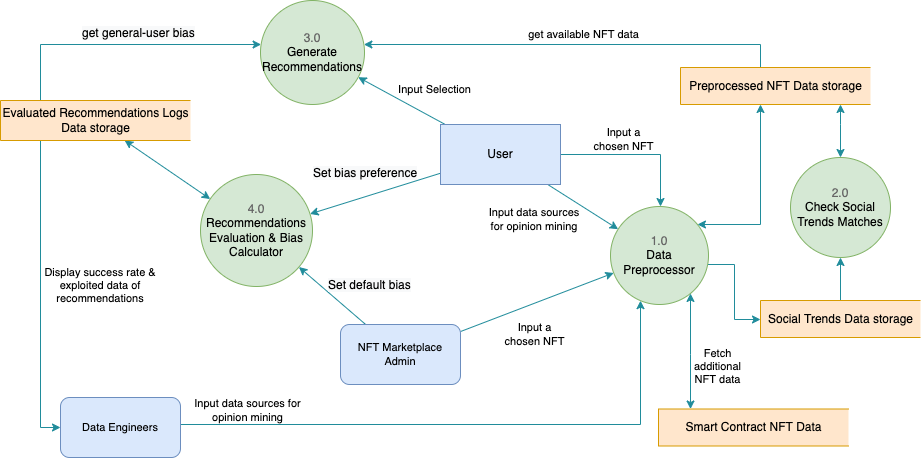
\includegraphics[width=0.95\textwidth]{images/Design/Data Flow Diagram L1.png}}
% https://tex.stackexchange.com/a/423679
\caption{Data Flow Diagram - Level 1 \textit{(self-composed)}}
\label{fig:data-flow-diagram-l1}
\end{figure}


% Add a L2 Data flow diagram, if there's space left
\noindent The Level 2 Data Flow Diagram presented below provides a more extensive breakdown of the components of the above Level 1 Data Flow Diagram.

% drawio file: https://drive.google.com/file/d/1XFBAVPGVhEBqQPh0X6YoGenb3icNOS3I/view?usp=sharing

\begin{figure}[h!]
\centering
\setlength{\fboxsep}{10pt}%
\setlength{\fboxrule}{0.5pt}%
\fbox{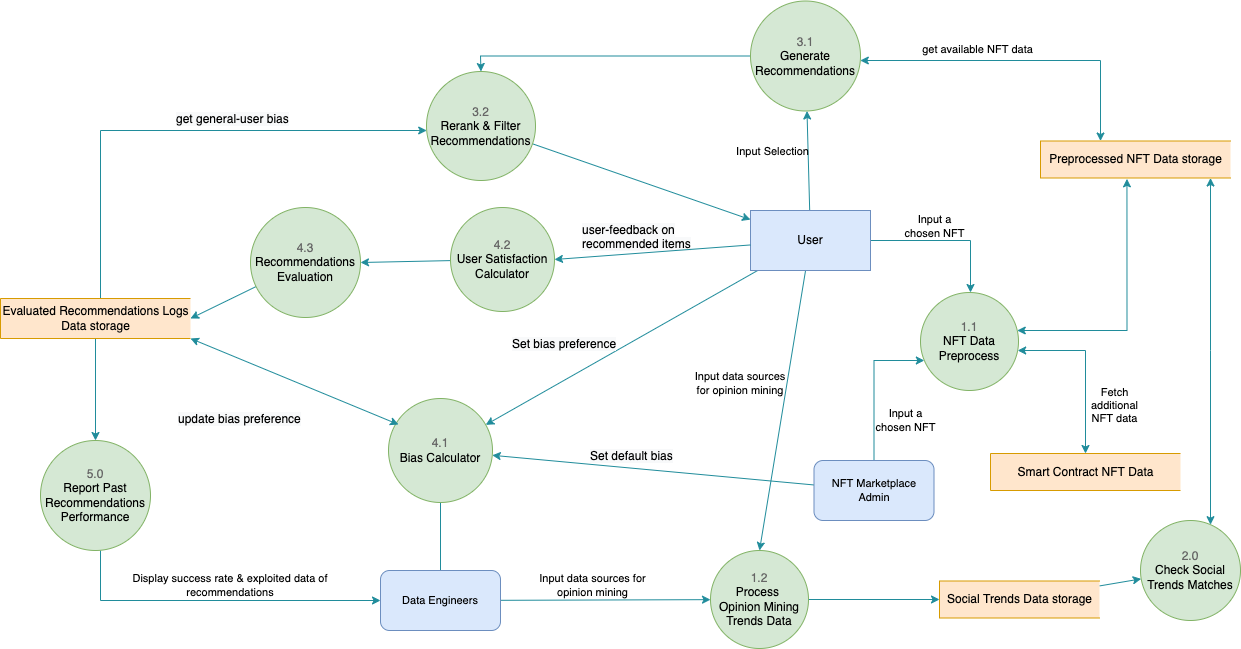
\includegraphics[width=0.95\textwidth]{images/Design/Data Flow Diagram L2.png}}
% https://tex.stackexchange.com/a/423679
\caption{Data Flow Diagram - Level 2 \textit{(self-composed)}}
\label{fig:data-flow-diagram-l2}
\end{figure}

\subsection{Algorithm Design}

When studying available data in the system, it was identified that cross-collection \gls{nft}s cannot be recommended using the same concepts \& data points followed for inter-collection matches. Therefore, multiple algorithms were considered to get a diverse set of recommendations.

\subsubsection{Infusing trends matches into Recommendations}
% >>social-trends calculation (tweet-volume/ same info in multiple sources) and matches
The equation composed below is designed to be used to calculate the total trends score for an item. The methods of utilization of this score for recommendations have been discussed following the breakdown of the equation.

% \vspace{4mm}
% algorithm
\begin{figure}[h!]
% \[
\begin{equation}
T_{t_{s},i} = \frac{\sum^{N_{i_{s}}}_{i_{s}=1} \left[\sum^{k_{w}}_{k_{w}=1} s_{c} \left(\frac{t_{vt,c}}{Med(T_{vt})}\right) \frac{m u}{\left(\mu + n_{m}\right)} \right]}{N_{i_{s}}}
\end{equation}
% \]
\caption*{Equation for social trend-match score for recommendations \textit{(self-composed)}}
\end{figure}

% describe algorithm
\noindent$T_{t_{s},i}$ - Total trends score for one item\\
$N_{i_{s}}$ - Total number of information sources\\
$i_{s}$ - Source of information\\
$k_{w}$ - Number of keywords in the current item\\
$s_{c}$ - Sentiment score surrounding chosen trend content\\
$m$ - Match value, a Boolean used to check if the current evaluated content contains the chosen trend to be matched against. \\
$u$ - User priority, used to check the current user's interest in the chosen trend. This is 1 by default\\
$t_{vt,c}$ - Tweet volume at this moment in time of the chosen content \\
$Med(T_{vt})$ - Median Tweet volume at this moment in time\\
$\mu$ - Constant, set to 0.1 to avoid division by 0 error for today's trends\\
$n_{m}$ - Number of days between the current day \& the day of the trend.\\

\noindent The following equation extracts the calculation of the impact score of the chosen trend ($i_{t}$), as described above. Twitter data has been taken as the example source here. The data source can be even an internet forum.
\begin{figure}[h!]
\begin{equation}
i_{t} = \frac{t_{vt,c}}{Med(T_{vt})}
\end{equation}
\caption*{Equation for the calculation of the impact score of a chosen trend \textit{(self-composed)}}
\end{figure}

For trends that don't have a measurable volume, $t_{vt,c}$ can be taken as $\left(T_{vt}{min} - 1\right)$ to give it the lowest possible value, or as $Med(T_{vt})$ to omit the impact score all-together.

\bigbreak
The algorithm, $T_{t_{s},i}$ can be applied to inter-collection recommendations as well, if each \gls{nft} in the collection has unique names and descriptions. Using unique traits didn't seem to make sense for comparison with this algorithm, but it may be valid if it can be proved that the traits can be matched with trends data.

The Total trends score for one item calculated above can either be taken for recommendations as to the top N items or as an absolute similarity match with other chosen items' trends scores.

\bigbreak
The beauty of this equation is that it isn't necessarily required to be applied for only \gls{nft} recommendations. It can be used to enhance any content-based recommendations model. It can be seen as another way of infusing collaborative filtering, without the collection of user-specific data by the platform that integrates the presented Recommendations Architecture.

% mention these and how they get enhanced with the designed algorithm
% these aren't created algorithms: >basic content based recommendations >consider owner-clustering (giving scores to this may be considerable as an overview algorithm for design)

\subsubsection{Recommendations based on Rarity}
% same-collection
% >>TODO:Add this to LR!!! total-rarity calculation
% 

\begin{figure}[h!]
\begin{equation}
T_{r,t} = \sum^{Nt}_{t=1} \frac{1}{\left(\frac{c_{t}}{T_{N}}\right)}
\end{equation}
\caption*{Equation for the calculation of the total trait rarity score of an \gls{nft} \textit{()}}
\end{figure}

\noindent$T_{r,t}$ - Total rarity of a trait\\
$Nt$ - Total number of traits in the \gls{nft}\\
$c_{t}$ - Trait count of the chosen trait (number of occurrences in the collection)
$T_{N}$ - Total supply of \gls{nft}s in the collection

The absolute difference between the total rarities is calculated when an \gls{nft} from a collection is chosen. The lowest scoring items are recommended to the user. This gives the \gls{nft}s that may be as closely valuable as the initially chosen \gls{nft}. This allows recommending \gls{nft}s that don't have unique content descriptions.

Furthermore, the traits are fed into a Content-based Recommendations Model to get \gls{nft}s with the most similar traits to be recommended.


% mention these and how they get enhanced with the designed algorithm
% these aren't created algorithms: >traits-based matches >consider creator-clustering (giving scores to this may be considerable as an overview algorithm for design)



% \bigbreak
% >>using a varying bias instead of weighted bias for diversity in recommendations
\subsubsection{Varying Bias for Recommendations Diversifier}
Finally, all these recommendations produced by algorithmic models had to be presented to the user suitably. Instead of going with a weighted bias which was recommended by the experts that were interviewed, it was decided to make this bias variable with time. 

The reason for opting for this in contrast to having pre-trained weights \& biases using a Neural Network architecture that Amazon successfully attempted with its recent Autoencoder \autocite{larry_history_2019} \gls{dl} model was to allow a more optimized output, without having to retrain the model. Another reason to opt for this method was due to the lack of user data to identify the most optimum weights or to train a \gls{dl} model.

The calculation of this bias draws concepts from Reinforcement learning techniques.
% >>calculating default bias
\begin{figure}[h!]
\begin{equation}
B_{w,p} = \frac{\left[ \sum^{n_{g}}_{i=0} \frac{b_{p,s}}{\left( \alpha + n_{m} \right)} \right]}{N_{n_{g}}} 
\end{equation}
\caption*{Equation for the calculation of the recommendations bias in combining outputs in ensembled models \textit{(self-composed)}}
\end{figure}

\noindent $B_{w,p}$ - Default Bias weighting for a chosen pipeline that recommendations are given from\\
$b_{p,s}$ - Successful bias selection for a chosen pipeline for the last n days\\
$\alpha$ - Constant, set to 0.001 to avoid division by 0 error for today's bias selections\\
$n_{m}$ - Number of days away from the current day.\\
$n_{g}$ - Grouped days (Eg: 1 day, 7 days, 1 month, 3 months, 6 months, 1 year)\\
$N_{n_{g}}$ - Total number of grouped days considered

% >Evaluating recommendations

% >how it's decided to push the recommendations towards admin's bias - this in turn may alter the default bias


\subsubsection{Applying Bias Push}

When presenting recommendations, the author decided to allow a system admin to be capable of suggesting a push towards a preferred direction to allow the bias to be altered.

\begin{figure}[h!]
\begin{equation}
B_{c,p} = b_{l,p} + \left( B_{w,p} - b_{a,p} \right)
\end{equation}
\caption*{Equation for the calculation of the recommendations bias in combining outputs in ensembled models \textit{(self-composed)}}
\end{figure}

\noindent$B_{c,p}$ - Current bias of a chosen recommendations pipeline\\
$b_{l,p}$ - Last applied user bias for the chosen recommendations pipeline. This can be 0 or null\\
$B_{w,p}$ - Default bias of a chosen recommendations pipeline\\
$b_{a,p}$ - Admin suggested bias of a chosen recommendations pipeline\\

The above bias will be applied only to users who haven't chosen a preferred bias. It can be applied to users who have chosen the bias as well, but it is suggested to be applied after initially showing recommendations to the user using their requested bias.


\subsection{UI Design}
% low fidelity wireframes
UI wireframes will be designed and added before implementing the UI of the MVP (Minimum Viable Product) that will be created over the following weeks. Since the core research component didn't require a UI, this design was not necessary for this submission.

% \pagebreak
\subsection{System Process Flow Chart}
The algorithm's flow and decision structures are depicted in the flowchart below. It explains a significant proportion of the system since the expected implementation is primarily procedural.

% might have to show this page in landscape orientation
\begin{figure}[h!]
\centering
\setlength{\fboxsep}{10pt}%
\setlength{\fboxrule}{0.5pt}%
\fbox{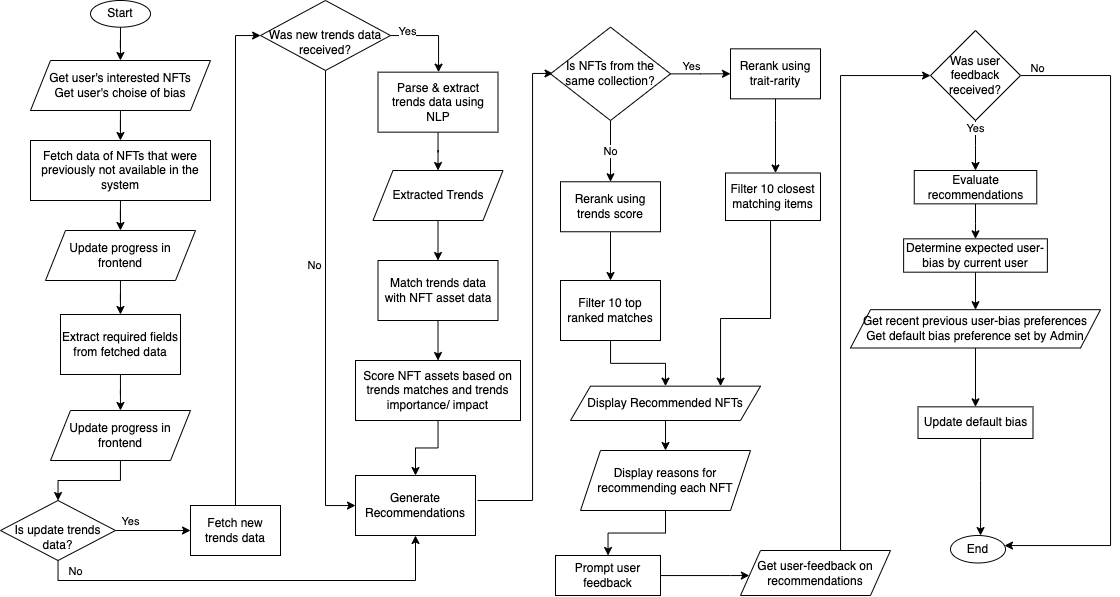
\includegraphics[width=0.95\textwidth]{images/Design/System Process Flow Chart.png}}
\caption{System Process Flow Chart\textit{(self-composed)}}
\label{fig:system-process-flowchart}
\end{figure}

% TODO: add price prediction, evaluation & bias altering based on feedback to flow chart

\section{Chapter Summary}
The design, architectural aspects, and the flow of the project and novel author-designed algorithms were documented in this chapter followed by the expected UI wireframes to be implemented for the end-users interaction with the system.
